\documentclass[]{article}
\usepackage{lmodern}
\usepackage{amssymb,amsmath}
\usepackage{ifxetex,ifluatex}
\usepackage{fixltx2e} % provides \textsubscript
\ifnum 0\ifxetex 1\fi\ifluatex 1\fi=0 % if pdftex
  \usepackage[T1]{fontenc}
  \usepackage[utf8]{inputenc}
\else % if luatex or xelatex
  \ifxetex
    \usepackage{mathspec}
  \else
    \usepackage{fontspec}
  \fi
  \defaultfontfeatures{Ligatures=TeX,Scale=MatchLowercase}
\fi
% use upquote if available, for straight quotes in verbatim environments
\IfFileExists{upquote.sty}{\usepackage{upquote}}{}
% use microtype if available
\IfFileExists{microtype.sty}{%
\usepackage{microtype}
\UseMicrotypeSet[protrusion]{basicmath} % disable protrusion for tt fonts
}{}
\usepackage[margin=1in]{geometry}
\usepackage{hyperref}
\hypersetup{unicode=true,
            pdftitle={CSC2506 Assignment 2},
            pdfauthor={Matthew Scicluna},
            pdfborder={0 0 0},
            breaklinks=true}
\urlstyle{same}  % don't use monospace font for urls
\usepackage{graphicx,grffile}
\makeatletter
\def\maxwidth{\ifdim\Gin@nat@width>\linewidth\linewidth\else\Gin@nat@width\fi}
\def\maxheight{\ifdim\Gin@nat@height>\textheight\textheight\else\Gin@nat@height\fi}
\makeatother
% Scale images if necessary, so that they will not overflow the page
% margins by default, and it is still possible to overwrite the defaults
% using explicit options in \includegraphics[width, height, ...]{}
\setkeys{Gin}{width=\maxwidth,height=\maxheight,keepaspectratio}
\IfFileExists{parskip.sty}{%
\usepackage{parskip}
}{% else
\setlength{\parindent}{0pt}
\setlength{\parskip}{6pt plus 2pt minus 1pt}
}
\setlength{\emergencystretch}{3em}  % prevent overfull lines
\providecommand{\tightlist}{%
  \setlength{\itemsep}{0pt}\setlength{\parskip}{0pt}}
\setcounter{secnumdepth}{0}
% Redefines (sub)paragraphs to behave more like sections
\ifx\paragraph\undefined\else
\let\oldparagraph\paragraph
\renewcommand{\paragraph}[1]{\oldparagraph{#1}\mbox{}}
\fi
\ifx\subparagraph\undefined\else
\let\oldsubparagraph\subparagraph
\renewcommand{\subparagraph}[1]{\oldsubparagraph{#1}\mbox{}}
\fi

%%% Use protect on footnotes to avoid problems with footnotes in titles
\let\rmarkdownfootnote\footnote%
\def\footnote{\protect\rmarkdownfootnote}

%%% Change title format to be more compact
\usepackage{titling}

% Create subtitle command for use in maketitle
\newcommand{\subtitle}[1]{
  \posttitle{
    \begin{center}\large#1\end{center}
    }
}

\setlength{\droptitle}{-2em}
  \title{CSC2506 Assignment 2}
  \pretitle{\vspace{\droptitle}\centering\huge}
  \posttitle{\par}
  \author{Matthew Scicluna}
  \preauthor{\centering\large\emph}
  \postauthor{\par}
  \predate{\centering\large\emph}
  \postdate{\par}
  \date{2017-01-13}

\usepackage{amsmath}
\usepackage {tikz}
\usetikzlibrary{arrows.meta}

\begin{document}
\maketitle

\section{Graphical model
distributions}\label{graphical-model-distributions}

\subsection{Directed Graph}\label{directed-graph}

\begin{enumerate}
\def\labelenumi{\arabic{enumi}.}
\item
  The statement MUST BE TRUE. We show that \(x_4\) is d-seperated from
  \(x_5\) conditioned on
  \(x_3 \Rightarrow x_4 \perp x_5 \mid x_1, x_2, x_3\). This is clear
  though since there are only 2 paths, so we just have to check them
  both. \(x_4 \rightarrow x_6 \rightarrow x_5\) doesn't work since
  \(x_6\) explains away \(x_4\) and \(x_5\).
  \(x_4 \rightarrow x_3 \rightarrow x_5\) doesn't work either since
  \(x_3\) is the common cause of \(x_4\) and \(x_5\).
\item
  The statement MUST BE TRUE. Once again we show that \(x_3\) is
  d-seperated from \(x_7\) conditioned on \(x_4\) and \(x_5\). There are
  only two paths to check,
  \(x_3 \rightarrow x_4 \rightarrow x_6 \rightarrow x_7\) and
  \(x_3 \rightarrow x_5 \rightarrow x_6 \rightarrow x_7\). \(x_4\) and
  \(x_5\) block each path respectively as they are being conditioned on
  and they form chains between \(x_3\) and \(x_6\).
\item
  The statement MUST BE TRUE. There is only 1 path
  \(x_1 \rightarrow x_3 \rightarrow x_2\) which is blocked since \(x_3\)
  and all of its is descendants are not conditioned on, meaning it
  explains away \(x_1\) and \(x_2\).
\item
  The statement COULD BE TRUE. We can only determine that \(x_4\) and
  \(x_5\) are not d-connected, but this is not sufficient to conclude
  that they are not independant. To show that \(x_4\) and \(x_5\) are
  not d-connected, take the path
  \(x_4 \rightarrow x_6 \rightarrow x_5\).
\end{enumerate}

\subsection{Undirected Graph}\label{undirected-graph}

\begin{enumerate}
\def\labelenumi{\arabic{enumi}.}
\item
  The statement CANNOT BE TRUE. It is enough to find a path from \(x_4\)
  to \(x_5\) that doesn't pass through \(x_1\), \(x_2\) or \(x_3\). One
  such path is \(x_4 \rightarrow x_7 \rightarrow x_5\).
\item
  The statement MUST BE TRUE. Every path between \(x_3\) and \(x_7\)
  passes through either \(x_4\) or \(x_5\).
\item
  The statement CANNOT BE TRUE. \(x_1\) and \(x_2\) share an edge and so
  cannot be independant!
\item
  The statement CANNOT BE TRUE. A path that goes from \(x_4\) to \(x_5\)
  without passing \(x_3\) or \(x_6\) is
  \(x_4 \rightarrow x_7 \rightarrow x_5\)
\end{enumerate}

\newpage

\section{Complete graphs}\label{complete-graphs}

\begin{enumerate}
\def\labelenumi{\arabic{enumi}.}
\tightlist
\item
  Consider the following 5 variables ordered arbitrarily as \(x_1\),
  \(x_2\), \(x_3\), \(x_4\), and \(x_5\). We wish to draw a directed
  graphical model which can capture any joint distribution and is
  acyclic. This means that we want our graph to capture the following
  dependancy:
\end{enumerate}

\begin{align*}
p(x_1, x_2, x_3, x_4, x_5) &= p(x_1)P(x_2 \mid x_1)p(x_3 \mid x_2, x_1)p(x_4 \mid x_3, x_2, x_1)p(x_5 \mid x_4, x_3, x_2, x_1) 
\end{align*}

From this we see we must capture all the pairwise dependancies:
\(P(x_i \mid x_j) \quad \forall i > j \in \left\{ {1, 2, 3, 4, 5}\right\}\)

We see that the following graph models this dependancy, given our
ordering.

\begin{tikzpicture}
\begin{scope}[every node/.style={circle,thick,draw}]
    \node (A) at (6,2.5) {$x_1$};
    \node (B) at (2,0) {$x_2$};
    \node (C) at (10,0) {$x_3$};
    \node (D) at (4,-4) {$x_4$};
    \node (E) at (8,-4) {$x_5$};
\end{scope}

\begin{scope}[>={Stealth[black]},
              every node/.style={fill=white,circle},
              every edge/.style={draw=black,very thick}]
    \path [->] (A) edge node {$p(x_2 \mid x_1)$} (B);
    \path [->] (A) edge node {$p(x_3 \mid x_1)$} (C);
    \path [->] (A) edge node {$$} (D);
    \path [->] (A) edge node {$$} (E);
    
    \path [->] (B) edge node {$$} (C);
    \path [->] (B) edge node {$p(x_4 \mid x_2)$} (D);
    \path [->] (B) edge node {$$} (E);
    
    \path [->] (C) edge node {$$} (D);
    \path [->] (C) edge node {$p(x_5 \mid x_3)$} (E);
    
    \path [->] (D) edge node {$p(x_5 \mid x_4)$} (E);
    
\end{scope}
\end{tikzpicture}

\begin{enumerate}
\def\labelenumi{\arabic{enumi}.}
\setcounter{enumi}{1}
\item
  We see that no edges Can be added to this graph since it is complete
  (every pair of nodes is connected by an edge). If any edge is removed
  from this graph we see that we will be enforcing certain conditional
  independancies which would limit the class of distributions that this
  graph can convey. This is since it would only be able to model joint
  distributions with particular conditional independancies between the
  variables.
\item
  We seek to draw an undirected graphical model on four variables which
  can capture any joint distribution. We also want to list all the
  maximal cliques. Again we see that we need edges between every pair of
  vertices or else we will not be able to capture every possible joint
  distribution (since missing edges imply that we can only model joint
  distributions with conditional independances). We see the following
  graph satisfies this since it is complete. Note that this graph is
  complete meaning that it has exactly one maximal clique - the entire
  graph itself.
\end{enumerate}

\begin{tikzpicture}[auto, node distance=3cm, every loop/.style={},
                    thick,main node/.style={circle,draw,font=\sffamily\Large\bfseries}]

  \node[main node] (1) {$x_1$};
  \node[main node] (2) [below left of=1] {$x_2$};
  \node[main node] (3) [below right of=2] {$x_3$};
  \node[main node] (4) [below right of=1] {$x_4$};

  \path[every node/.style={font=\sffamily\small}]
    (1) edge node [left] {} (4)
        edge node [left] {} (3)
        edge node [left] {} (2)
        
    (2) edge node [right] {} (1)
        edge node {} (4)
        
    (3) edge node [right] {} (2)
    
    (4) edge node [left] {} (3);
\end{tikzpicture}

\begin{enumerate}
\def\labelenumi{\arabic{enumi}.}
\setcounter{enumi}{3}
\item
  Once again, no edges can be added since the graph is complete, and
  none can be removed or else the graph will not be able to model every
  possible joint distribution, and only ones with particular conditional
  independances between the variables.
\item
  {[}Bonus{]} The claim is TRUE. We prove it by showing that every
  graphical model which can capture any joint distribution must be
  complete and that a complete graph has \(\frac{k^2}{2} - \frac{k}{2}\)
  edges.
\end{enumerate}

\begin{itemize}
\item
  Firstly, if a graphical model is not complete than it will be missing
  edges \(\Rightarrow\) it can only model joint distributions with
  conditional independancies imposed between some of it's variables. So
  clearly the graph must be complete.
\item
  Secondly, a complete graph has edges between every possible pair of
  nodes. This means if the graph has k nodes it has \({k \choose 2}\)
  edges. Note that
  \({k \choose 2} = \frac{k!}{(k-2)!2} = \frac{k(k-1)}{2} = \frac{k^2}{2} - \frac{k}{2}\).
  So the claim holds, as needed.
\end{itemize}

\section{Learning Undirected Models}\label{learning-undirected-models}

We are given the following

\[p(x \mid \theta) = exp \biggl\{\sum_{s \in V}  \theta_{s}x_{s} + \sum_{(s,t) \in E} \theta_{st}x_{s}x_{t}-\Phi(\theta) \biggl\}\]

where

\[
\Phi(\theta) = log \biggl\{\sum_{x} exp \biggl\{\sum_{s \in V}  \theta_{s}x_{s} + \sum_{(s,t) \in E} \theta_{st}x_{s}x_{t} \biggl\} \biggl\}
\]

\subsection{MLE for Fully Disconnected pairwise binary
MRF}\label{mle-for-fully-disconnected-pairwise-binary-mrf}

Note that the maximum likelihood (ML) estimates of the node parameters
\(\theta_s\) when E = \(\emptyset\) is as follows:

\[
\ell(\theta \mid x) = ln p(x \mid \theta) = ln \biggl\{ exp \biggl\{\sum_{s \in V}  \theta_{s}x_{s} -\Phi(\theta) \biggl\} \biggl\} = \sum_{s \in V}  \theta_{s}x_{s} - \Phi(\theta)
\]

So for data points \(x_s^{(i)}\), \(i = 1, 2,\) \ldots{}\(N\), each with
features \(s = 1, 2,\)\ldots{}\(, k\).

\[  \frac{\partial \ell(\theta_s \mid x)}{\partial \theta_s} = \frac{\partial}{\partial \theta_s} \sum_{i=1}^{N} ln P(x_s^{(i)} \mid \theta) = \sum_{i=1}^{N} \frac{\partial}{\partial \theta_s}  \sum_{s \in V}  \theta_{s}x_{s}^{(i)} - \Phi(\theta) = 0\]

and using the linearity of the differentiation operator and that
\(\frac{\partial}{\partial \theta_s} \Phi(\theta) = E(x_s \mid \theta)\)
since \(x\) is in the exponential family we have that, after rearranging
terms:

\[
\bar{x_s} = \frac{1}{N} \sum_{i=1}^{N} x_{s}^{(i)} = E(x_s \mid \theta)
\]

Finally a plot of the \(\theta_s\) for each senator can be found in
figure 1.

\begin{figure}
\begin{center}
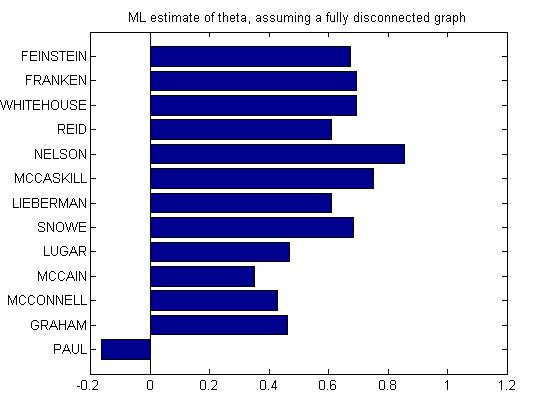
\includegraphics[width=250pt]{fig1.jpg}
\caption{Plot of each Senators theta parameter, assuming a fully disconnected graph}
\end{center}
\end{figure}

To compute the expectation we see that:

\begin{align*}
E(x_s \mid \theta) &= \sum_{x_s=0}^{1} \frac{exp( \sum_{i=1}^{13} x_i \theta_i) x_s}{\sum_{x_s=0}^{1} exp(\sum_{i=1}^{13} x_i \theta_i)} \\
&= \sum_{x_s=0}^{1} \frac{\prod_{j \ne s} exp( x_j \theta_j) exp( x_s \theta_s) x_s}{\sum_{x_s=0}^{1} \prod_{j \ne s} exp(x_i \theta_i) exp(x_s \theta_s)}\\
&= \sum_{x_s=0}^{1} x_s \frac{e^{x_s \theta_s}}{1+e^{x_s \theta_s}}  \\
&= \frac{e^{\theta_s}}{1+e^{\theta_s}}
\end{align*}

And combining this yields:

\[
\bar{x_s} = \frac{e^{\theta_s}}{1+e^{\theta_s}} \Rightarrow \theta_s = ln(  \frac{\bar{x_s}}{1 - \bar{x_s}} )
\]

\subsection{Gradient of the Log Likelihood of This
Model}\label{gradient-of-the-log-likelihood-of-this-model}

First we find the sufficient statistics. Using that \(x^{(i)}\) is from
the exponential family, we see that:

\begin{align*}
P(Data) &= \prod^{N}_{i=1} P(x^{(i)}) = \prod^{N}_{i=1} exp \biggl\{\sum_{s \in V}  \theta_{s}x_{s}^{(i)} - \sum_{(s,t) \in E}  \theta_{st} x_{s}^{(i)} x_{t}^{(i)}  - \Phi(\theta) \biggl\} \\
&= exp \biggl\{\sum_{i=1}^N \sum_{s \in V}  \theta_{s}x_{s}^{(i)} - \sum_{i=1}^N \sum_{(s,t) \in E}  \theta_{st} x_{s}^{(i)} x_{t}^{(i)}  - N \Phi(\theta) \biggl\} \\
&= exp \biggl\{ \sum_{s \in V}  \theta_{s} \sum_{i=1}^N x_{s}^{(i)} - \sum_{(s,t) \in E}  \theta_{st} \sum_{i=1}^N x_{s}^{(i)} x_{t}^{(i)}  - N \Phi(\theta) \biggl\}
\end{align*}

So the sufficient statistics are \(\sum_{i=1}^N x_{s}^{(i)}\) and
\(\sum_{i=1}^N x_{s}^{(i)} x_{t}^{(i)}\)

Now, given this we derive an expression for the gradient of this
log-likelihood with respect to \(\theta_s\) and \(\theta_{st}\)

For \(\theta_s\) we have that:

\begin{align*}
\frac{\partial \ell(\theta_s \mid x)}{\partial \theta_s} &= \frac{\partial}{\partial \theta_s} \sum_{i=1}^N \sum_{s \in V}  \theta_{s}x_{s}^{(i)} + \sum_{(s,t) \in E} \theta_{st}x_{s}^{(i)}x_{t}^{(i)}-\Phi(\theta) \\
&=\sum_{i=1}^N x_{s}^{(i)} - N E(X_s \mid \theta) \\
&=\sum_{i=1}^N x_{s}^{(i)} - N P(X_s = 1 \mid \theta)
\end{align*}

Since \(x_s \in \{0,1\}\)

For \(\theta_{st}\) we have that:

\begin{align*}
\frac{\partial \ell(\theta_{st} \mid x)}{\partial \theta_{st}} &= \frac{\partial}{\partial \theta_{st}} \sum_{i=1}^N \sum_{s \in V}  \theta_{s}x_{s}^{(i)} + \sum_{(s,t) \in E} \theta_{st}x_{s}^{(i)}x_{t}^{(i)}-\Phi(\theta) \\
&=\sum_{i=1}^N x_{s}^{(i)}x_{t}^{(i)} - N E(X_s X_t \mid \theta) \\
&=\sum_{i=1}^N x_{s}^{(i)}x_{t}^{(i)} - N P(X_s = 1 \cap X_t = 1 \mid \theta)
\end{align*}

\subsection{Computing ML Estimates of Model
Parameters}\label{computing-ml-estimates-of-model-parameters}

Using the above gradient objective formulas and the MATLAB optimization
package \(\texttt{L1General}\), we computed the ML estimates of a fully
connected pairwise graphical model. We used this on the full Senate
voting record. Figure 2 contains a plot the log-likelihood of the model
after each iteration.

\begin{figure}
\begin{center}
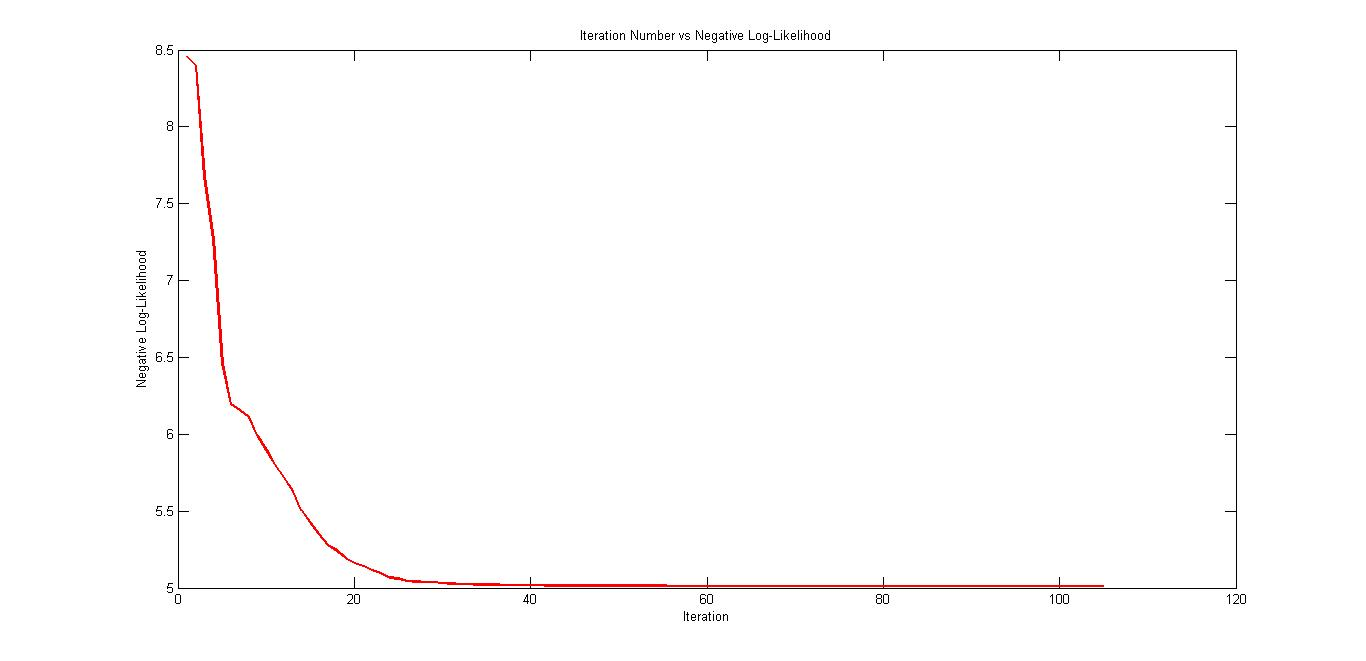
\includegraphics[width=250pt]{fig2.jpg}
\caption{Plot negative log-likelihood of fully connected model}
\end{center}
\end{figure}

\subsection{Representational Power of this
Model}\label{representational-power-of-this-model}

The fully connected, pairwise graphical model estimated cannot represent
any joint distribution on N binary variables? This is because it can
only capture pairwise dependancies, but not higher order ones. An
example of one such higher order dependancy is as follows: suppose
Senator Paul always voted with Senator Franken, provided Senator Reid
did too. Our pairwise model would be unable to capture this three-way
interaction.

\subsection{Binary Entropy Comparison}\label{binary-entropy-comparison}

We compared the factorized model and the fully connected model by
computing the binary entropy of each of the corresponding joint
distributions. We found that the binary entropy was 12.2 and 7.23
respectively. Since the difference is not that large, this suggests that
the voting patterns of Senators are largely unaffected by the voting
patterns of other Senators.

\subsection{Using Factorized Laplacian
Priors}\label{using-factorized-laplacian-priors}

We explore what happens when we put a Laplacian prior on each
\(\theta_s\) and \(\theta_{s,t}\). The prior has the following form:

\[P(\theta \mid \lambda) =  \prod_{s \in V}  \frac{\lambda_s}{2}e^{(-\lambda_s \mid \theta_s  \mid)} \prod_{(s,t) \in E} \frac{\lambda_{st}}{2}e^{(-\lambda_{st} \mid \theta_{st}  \mid)}\]

We see that:

\begin{align*}
\ell(\theta \mid x, \lambda) &= \sum_{i=1}^N ln P(x^{(i)} \mid \theta, \lambda) \\
&= \sum_{i=1}^N ln P(x^{(i)} \mid \theta) + ln P(\theta \mid \lambda) \\
&= \sum_{i=1}^N ln P(x^{(i)} \mid \theta) + \sum_{s \in V}  log \left( \frac{\lambda_s}{2} \right) -\lambda_s \mid \theta_s \mid + \sum_{(s,t) \in E} log \left( \frac{\lambda_{st}}{2} \right) -\lambda_{st} \mid \theta_{st}  \mid \\
&\propto \sum_{i=1}^N ln P(x^{(i)} \mid \theta) - \bar {\lambda } \sum_{(s,t) \in E} \mid \theta_{st}  \mid
\end{align*}

Note that the last step follows if we impose the contstraints that
\(\lambda_s \rightarrow 0\) and \(\lambda_{st} = \bar {\lambda }\).

\subsection{Comparing Different Values of Our L1 Penalization
Term}\label{comparing-different-values-of-our-l1-penalization-term}

From the above we saw that, given \(\lambda_s \rightarrow 0\) and
\(\lambda_{st} = \bar {\lambda }\), adding the Laplacian prior is
equivalent to adding an identical L1 regularization penalty term on each
of the \(\lambda_{st}\) terms. We used the votes for the first 400 bills
as a training set, and the remaining 86 bills as a validation set to
train seperate ising models, varying the value of \(\bar {\lambda }\).
We evaluated the log-probability of the validation data, and plotted
this in figure 3.

\begin{figure}
\begin{center}
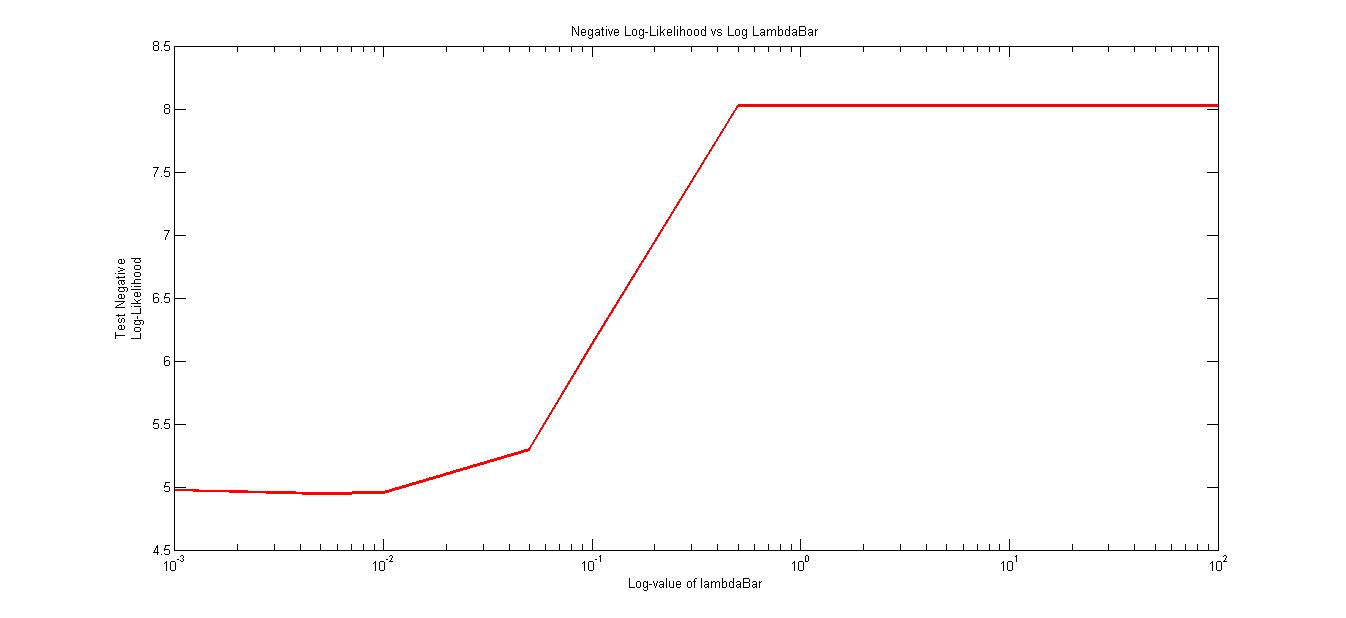
\includegraphics[width=400pt]{fig3.jpg}
\caption{Plot of negative log-likelihood vs Log Value of Theta Bar Hyperparameter}
\end{center}
\end{figure}

\newpage

\subsection{Associating Graphical
Structures}\label{associating-graphical-structures}

We notice that setting \(\bar{\lambda}\) = 0.5 gave the model which
produced the highest validation log-likelihood, and that
\(\bar{\lambda}\) = 0.1 gave the graph with the smallest number of edges
that was nevertheless connected. One way we could associate graphical
structures to the models learned is by using the \(\texttt{drawlayout}\)
function. This function creates a graph with distances of nodes based on
the value of the \(\theta\) parameters between the senators. We plot the
aformentioned models in figures 4 and 5 respectively.

It is interesting to note that upon \(\ell^1\) regularization, edges are
maintained disproportionately along party lines. This means that
senators tend to vote along party lines, with the noticable exception of
Senator Paul. Anyone who follows politics will notice that this isn't
surprising, since this is something he is known for.

\begin{figure}
\begin{center}
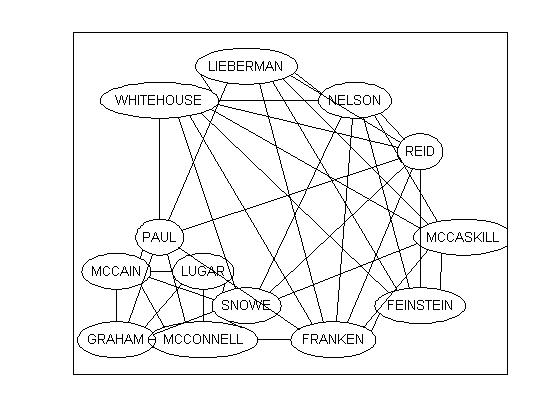
\includegraphics[width=200pt]{fig4.jpg}
\caption{Graph which produced the highest validation log-likelihood}
\end{center}
\end{figure}

\begin{figure}
\begin{center}
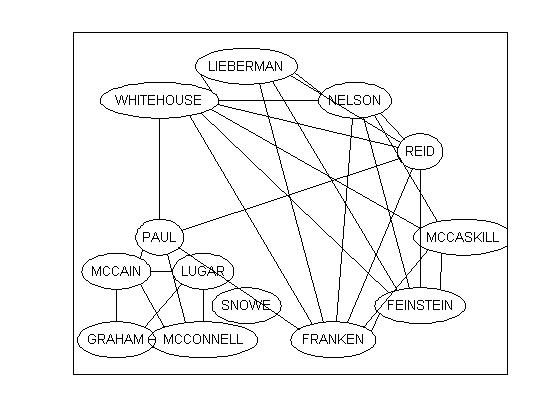
\includegraphics[width=200pt]{fig5.jpg}
\caption{Graph with the smallest number of edges that was nevertheless connected}
\end{center}
\end{figure}


\end{document}
